%===============================================================================
\begin{frame}[t]
\frametitle{Реализация LST-1 на FPGA}
    \begin{block}{\centering Реализация LST-1 на FPGA}
        \centering 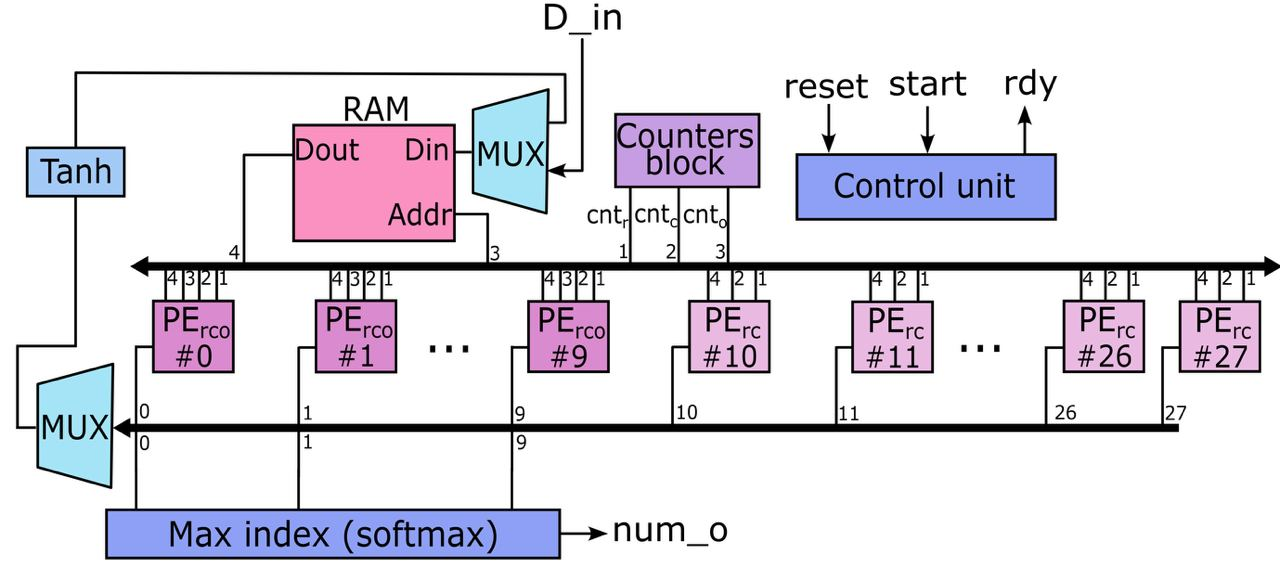
\includegraphics[width = 0.9\textwidth]{pics/impl1.jpg}
    \end{block}
\end{frame}
%===============================================================================
\begin{frame}[t]
    \frametitle{Реализация LST-1 на FPGA}
        \begin{block}{\centering Структура блоков PE}
            \centering 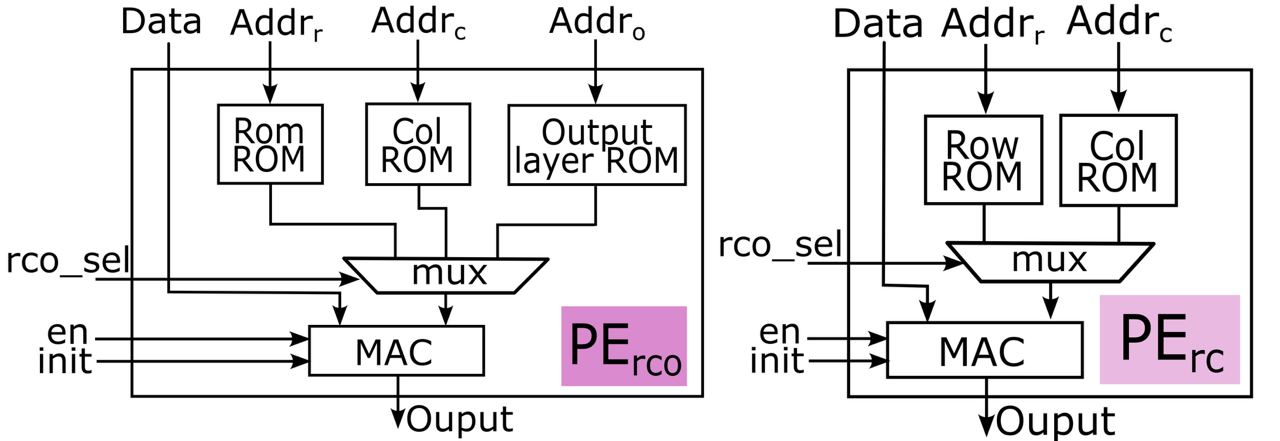
\includegraphics[width = 0.9\textwidth]{pics/pe.jpg}
        \end{block}
\end{frame}
%===============================================================================
\begin{frame}[t]
    \frametitle{Результаты синтеза}
    \begin{itemize}
        \item Вычислитель LST-1 описан на языке \textbf{SystemVerilog} и реализован на отладочной плате \textbf{Xilinx Zybo Z7 (FPGA XC7Z010)}.
        \item Для организации процесса тестирования использовался дистрибутив Linux \textbf{PYNQ}, который запускался на \textbf{ARM} ядре кристалла \textbf{XC7Z010}.
        \item Вычислитель LST-1 был реализован в виде IP-ядра с использованием \textbf{13-разрядного представления чисел}.
    \end{itemize}
    
    \vspace{1em}
    
    \begin{center}
    \begin{tabular}{|>{\raggedright\arraybackslash}p{4cm}|>{\centering\arraybackslash}p{3cm}|>{\centering\arraybackslash}p{3cm}|>{\centering\arraybackslash}p{3cm}|}
    \hline
    \textbf{Тип блока} & \textbf{Использовано} & \textbf{Доступно} & \textbf{Соотношение, \%} \\
    \hline
    LUT as logic & 1356 & 17600 & 7{,}7 \\
    \hline
    Flip Flop & 414 & 35200 & 1{,}2 \\
    \hline
    RAMB18 & 33 & 120 & 55{,}0 \\
    \hline
    DSP & 57 & 80 & 71{,}3 \\
    \hline
    \end{tabular}
    \end{center}
\end{frame}
